\documentclass[11pt]{article}
% Shared preamble for the printable mini lessons (1.4 onward).
%   \documentclass[11pt]{article}
%   \input{../preamble}
% Build the key with:  pdflatex -jobname=<name>_KEY "\def\iskey{}\input{<name>}"
% Figures shared with the web page live in figures/Unit_X/<name>.tex and are
% pulled in with \fig{Unit_X/<name>}; the standalone package drops their own
% preamble, so their macros come from figures/preamble.tex, loaded here.
% Shared preamble for web figures.  Each figure is a standalone .tex that
% \input's this file; scripts/make-figures.sh turns it into an SVG.
\usepackage[T1]{fontenc}
\usepackage{helvet}
\renewcommand{\familydefault}{\sfdefault}
\usepackage{tikz}
\usetikzlibrary{decorations.pathreplacing}
% axis numbers in the text font, not math italic
\pgfkeys{/pgf/number format/.cd,assume math mode=true,1000 sep={}}

% dot plot: \dotplot{min}{max}{value/count,...}{axis label}
\newcommand{\dotplot}[4]{%
\begin{tikzpicture}[x=0.9cm,y=0.33cm]
  \draw[thick] (#1-0.5,0) -- (#2+0.5,0);
  \foreach \t in {#1,...,#2} {\draw (\t,0.25) -- (\t,-0.25) node[below] {\t};}
  \foreach \v/\c in {#3} {\ifnum\c>0 \foreach \k in {1,...,\c} {\fill (\v,\k*1.15) circle (0.16cm);}\fi}
  \node at ({(#1+#2)/2},-2.3) {#4};
\end{tikzpicture}}

% shape sketch histogram (12 bins): \shapehist{heights}{label}
\newcommand{\shapehist}[2]{%
  \foreach \h [count=\i from 0] in {#1} \draw[fill=gray!30] (\i,0) rectangle (\i+1,\h);
  \draw (-0.3,0) -- (12.3,0);
  \node[font=\bfseries] at (6,-2.6) {#2};}
\newcommand{\meanmark}[1]{\fill (#1,0) -- ++(-0.3,-0.75) -- ++(0.6,0) -- cycle;}
\newcommand{\medmark}[2]{\draw[very thick,dashed] (#1,0) -- (#1,#2);}

% number line with minor ticks: \nline{min}{max}{label step}{axis label}
\newcommand{\nline}[4]{%
  \draw[thick] (#1-0.5,0) -- (#2+0.5,0);
  \foreach \t in {#1,...,#2} \draw (\t,0.12) -- (\t,-0.12);
  \pgfmathtruncatemacro{\nxt}{#1+#3}
  \foreach \t in {#1,\nxt,...,#2} \draw (\t,0.2) -- (\t,-0.2) node[below] {\t};
  \node at ({(#1+#2)/2},-0.95) {#4};}
% box plot above the line: \bplot{min}{Q1}{med}{Q3}{max}
\newcommand{\bplot}[5]{%
  \draw[thick] (#1,1.0) -- (#2,1.0);
  \draw[thick] (#4,1.0) -- (#5,1.0);
  \draw[thick] (#1,0.75) -- (#1,1.25);
  \draw[thick] (#5,0.75) -- (#5,1.25);
  \draw[thick,fill=gray!20] (#2,0.55) rectangle (#4,1.45);
  \draw[very thick] (#3,0.55) -- (#3,1.45);}

% ---- added for 1.4 onward ----
% axis on y=0: \axis{min}{max}{label step}{tick step}{axis label}
\newcommand{\axis}[5]{%
  \draw[thick] (#1,0) -- (#2,0);
  \pgfmathsetmacro{\axT}{#1+#4}\foreach \t in {#1,\axT,...,#2} \draw (\t,0.1) -- (\t,-0.1);
  \pgfmathsetmacro{\axL}{#1+#3}\foreach \t in {#1,\axL,...,#2}
    \draw (\t,0.18) -- (\t,-0.18) node[below] {\pgfmathprintnumber{\t}};
  \node at ({(#1+#2)/2},-0.95) {#5};}
% box plot centred at height y: \bplotat{y}{min}{Q1}{med}{Q3}{max}
\newcommand{\bplotat}[6]{%
  \draw[thick] (#2,#1) -- (#3,#1);
  \draw[thick] (#5,#1) -- (#6,#1);
  \draw[thick] (#2,#1-0.22) -- (#2,#1+0.22);
  \draw[thick] (#6,#1-0.22) -- (#6,#1+0.22);
  \draw[thick,fill=gray!20] (#3,#1-0.42) rectangle (#5,#1+0.42);
  \draw[very thick] (#4,#1-0.42) -- (#4,#1+0.42);}
% an outlier dot: \outlier{x}{y}
\newcommand{\outlier}[2]{\fill (#1,#2) circle (2.4pt);}

\usepackage[margin=0.75in]{geometry}
\usepackage{array}
\usepackage{enumitem}
\usepackage{amsmath}
\usepackage[helvet]{sfmath}  % math in the same sans font as the text
\usepackage{standalone}
\pagestyle{empty}
\setlength{\parindent}{0pt}
\setlist[enumerate,1]{leftmargin=1.5em,itemsep=1em}
\setlist[enumerate,2]{label=(\alph*),leftmargin=2em,itemsep=2.2em}

\newif\ifkey
\ifdefined\iskey \keytrue \fi
\colorlet{keyred}{red!75!black}
\newcommand{\ans}[1]{\ifkey\leavevmode{\color{keyred}#1}\fi}
% vertical work space on the student copy, less on the key
\newcommand{\work}[1]{\ifkey\vspace{0.6em}\else\vspace{#1}\fi}
\newcommand{\fig}[1]{\input{../../figures/#1}}
% Title line: \lessontitle{Quartiles, IQR, and Box Plots}
\newcommand{\lessontitle}[1]{{\Large\bfseries #1\ifkey\ \textcolor{keyred}{KEY}\fi}\hfill Name \underline{\hspace{2in}}\par\vspace{0.6em}}
\newcommand{\partner}{\par\vspace{0.4em}Work with a partner. Compare answers when you finish each problem.\par}

% Unit 1 test: four questions, one page and one data set each, so a mistake
% on one question does not carry into the next.
% Q2 data: Q1, median and Q3 are whole numbers (6th = 7th, 19th = 20th values).
% Q4 box plot is drawn from 3,5,7,8,9,10,10,11,12,13,13,14,14,14,15,16,17,18,
% 20,20,22,24,27,30,32 (6th = 7th, 13th = 14th, 19th = 20th), so adding 60
% really does leave Q1, the median and Q3 the same.
% The key keeps every box the same height as the student copy, so key page N
% lines up with test page N.
\newcommand{\goal}[1]{\textbf{#1}\par\vspace{0.35em}}
% answer box: same height on both copies, answer printed only on the key
\newcommand{\abox}[2]{\par\begin{minipage}[t][#1][t]{\linewidth}\raggedright\vspace{0.2em}\ans{#2}\end{minipage}\par}
% circled choices: \opt{A} prints plain; \optans{B} is circled in red on the key
\newcommand{\opt}[1]{\tikz[baseline=(c.base)]\node[rounded corners=0.6em,inner sep=2.5pt](c){#1};}
\newcommand{\optans}[1]{\ifkey\tikz[baseline=(c.base)]\node[rounded corners=0.6em,inner sep=2.5pt,draw=keyred,thick,text=keyred](c){#1};\else\opt{#1}\fi}
% five-number summary blanks, filled in red on the key
\newcommand{\fsblank}[1]{\underline{\makebox[0.65in]{\ans{#1}}}}
\newcommand{\fivesum}[5]{\par Min \fsblank{#1}\quad Q1 \fsblank{#2}\quad Median \fsblank{#3}\quad Q3 \fsblank{#4}\quad Max \fsblank{#5}\par}
\setlist[enumerate,2]{label=(\alph*),leftmargin=2em,itemsep=0.3em}
\setlist[enumerate,1]{leftmargin=1.5em,itemsep=1em}
\raggedright\hyphenpenalty=10000\exhyphenpenalty=10000

% dot plot with every whole number labelled, longer ticks at multiples of 5:
% \dplot{x scale}{min}{max}{value/count,...}{axis label}
\newcommand{\dplot}[5]{%
\begin{center}
\begin{tikzpicture}[x=#1,y=0.33cm]
  \draw[thick] (#2-0.5,0) -- (#3+0.5,0);
  \foreach \t in {#2,...,#3} {\draw (\t,0.22) -- (\t,-0.22) node[below,font=\footnotesize] {\t};
    \pgfmathtruncatemacro{\r}{mod(\t,5)}\ifnum\r=0 \draw[thick] (\t,0.4) -- (\t,-0.22);\fi}
  \foreach \v/\c in {#4} {\foreach \k in {1,...,\c} {\fill (\v,\k*1.1) circle (0.14cm);}}
  \node at ({(#2+#3)/2},-2.7) {#5};
\end{tikzpicture}
\end{center}}

\begin{document}

\lessontitle{Unit 1 Test: Displaying One Variable}

Show your work.

\begin{enumerate}

% ======================================================================
\item \goal{I make a histogram.}
A class grew 25 bean plants. The dot plot shows the height of each plant.
\dplot{0.55cm}{10}{40}{11/1,13/1,15/1,16/1,18/1,19/1,20/2,21/1,22/2,23/1,24/2,25/2,26/1,27/1,28/1,29/1,30/1,31/1,33/1,35/1,38/1}{Height (centimeters)}
\begin{enumerate}
  \item Make a frequency table. Count how many plants are in each group. Remember the histogram rule.

  \vspace{0.3em}
  \begin{center}
  \renewcommand{\arraystretch}{1.55}
  \begin{tabular}{|c|p{3.4in}|} \hline
  Height & Frequency \\ \hline
  10 to 15 & \ans{2 \;(11, 13)} \\
  15 to 20 & \ans{4 \;(15, 16, 18, 19)} \\
  20 to 25 & \ans{8 \;(20, 20, 21, 22, 22, 23, 24, 24)} \\
  25 to 30 & \ans{6 \;(25, 25, 26, 27, 28, 29)} \\
  30 to 35 & \ans{3 \;(30, 31, 33)} \\
  35 to 40 & \ans{2 \;(35, 38)} \\ \hline
  \end{tabular}
  \end{center}

  \item Make a histogram. Label both axes.

  \vspace{0.3em}
  \begin{center}
  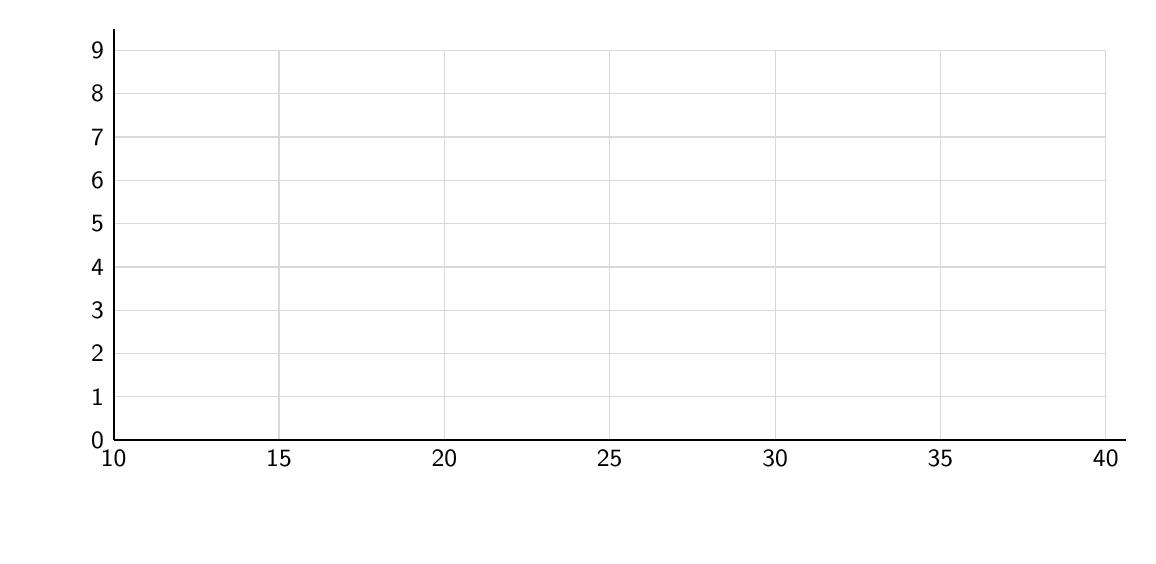
\begin{tikzpicture}[x=0.42cm,y=0.55cm]
    \foreach \y in {1,...,9} \draw[gray!30] (10,\y) -- (40,\y);
    \foreach \x in {15,20,...,40} \draw[gray!30] (\x,0) -- (\x,9);
    \draw[thick] (10,0) -- (40.6,0); \draw[thick] (10,0) -- (10,9.5);
    \foreach \y in {0,...,9} \node[left,font=\small] at (10,\y) {\y};
    \foreach \x in {10,15,...,40} \node[below,font=\small] at (\x,0) {\x};
    \ifkey\begin{scope}[keyred]
      \foreach \i/\h in {0/2,1/4,2/8,3/6,4/3,5/2} \draw[thick,fill=red!12] (10+\i*5,0) rectangle (15+\i*5,\h);
      \node[rotate=90] at (8,4.5) {Number of plants};
      \node at (25,-1.8) {Height (centimeters)};
    \end{scope}\else\path (7.4,0) (10,-2.2);\fi
  \end{tikzpicture}
  \end{center}
\end{enumerate}

% ======================================================================
\newpage
\item \goal{I find the five-number summary, and I make a box plot.}
A store kept track of T-shirt sales for 25 days. The dot plot shows how many T-shirts it sold each day.
\dplot{0.62cm}{0}{25}{4/1,6/1,7/1,8/2,9/2,10/2,11/2,12/2,13/2,14/3,15/2,16/1,17/1,18/1,20/1,22/1}{T-shirts sold in one day}
\begin{enumerate}
  \item Find the five-number summary.
  \abox{10em}{$n = 25$. The median is the 13th value: 12. Leave it out.\\[0.4em]
  Lower half: the first 12 values. \; Q1 $= (9 + 9) \div 2 = 9$ \quad (6th and 7th values)\\[0.4em]
  Upper half: the last 12 values. \; Q3 $= (15 + 15) \div 2 = 15$ \quad (19th and 20th values)}
  \fivesum{4}{9}{12}{15}{22}
  \vspace{1.5em}
  \item Make a box plot.

  \vspace{0.5em}
  \begin{center}
  \begin{tikzpicture}[x=0.62cm,y=1cm]
    \axis{0}{25}{5}{1}{T-shirts sold in one day}
    \ifkey\begin{scope}[keyred]\bplotat{1.1}{4}{9}{12}{15}{22}\end{scope}\else\path (0,1.8);\fi
  \end{tikzpicture}
  \end{center}
\end{enumerate}

% ======================================================================
\newpage
\item \goal{I find the mean and the median, I tell the shape, and I choose the best measure of center.}
25 students took a quiz. The quiz had 20 points. The dot plot shows each student's score.
\dplot{0.75cm}{0}{20}{1/1,4/1,6/1,9/1,11/1,12/1,14/1,15/1,16/3,17/4,18/5,19/3,20/2}{Quiz score (points)}
\begin{enumerate}
  \item Find $\Sigma x$ and the mean, $\bar{x}$. \quad ($\Sigma$ means add up. $n$ is the number of values.)
  \abox{8em}{$\Sigma x = 1 + 4 + 6 + 9 + 11 + 12 + 14 + 15 + 3(16) + 4(17) + 5(18) + 3(19) + 2(20) = 375$\\[0.6em]
  $n = 25$, \quad $\bar{x} = \frac{\Sigma x}{n} = \frac{375}{25} = 15$ points}
  \item Find the median.
  \abox{4.5em}{$n = 25$. The median is the 13th value: 17 points.}
  \item Circle the shape of the data.

  \vspace{0.6em}
  \optans{skewed left}\hspace{1.2em}\opt{symmetric}\hspace{1.2em}\opt{skewed right}
  \vspace{1.6em}
  \item Which describes a typical score better, the mean or the median? Explain.
  \abox{7em}{The median. The data are skewed left. A few low scores (1, 4, 6) pull the mean down to 15. 18 of the 25 students scored 15 or more, so the mean is too low to be typical.}
\end{enumerate}

% ======================================================================
\newpage
\item \goal{I use the 1.5 $\times$ IQR rule to find outliers.}
The box plot shows how many text messages 25 students sent yesterday.

\vspace{0.4em}
\begin{center}
\begin{tikzpicture}[x=0.45cm,y=1cm]
  \axis{0}{35}{5}{1}{Text messages sent}
  \bplotat{1.1}{3}{10}{14}{20}{32}
\end{tikzpicture}
\end{center}

\vspace{0.4em}
One more student sent 60 text messages. Now there are 26 students.\\
Adding 60 does \textbf{not} change Q1, the median, or Q3.
\begin{enumerate}
  \item Find the IQR. Then find the lower fence and the upper fence.
  \abox{11em}{From the box plot: Q1 $= 10$, Q3 $= 20$\\[0.5em]
  IQR $= Q3 - Q1 = 20 - 10 = 10$\\[0.5em]
  $1.5 \times 10 = 15$\\[0.5em]
  Lower fence $= 10 - 15 = -5$ \qquad Upper fence $= 20 + 15 = 35$}
  \item Is 60 an outlier? Explain.
  \abox{5em}{Yes. 60 is above the upper fence, 35.}
  \item How would the box plot change? What would stay the same? You do not have to draw a new box plot.
  \abox{11em}{The box stays the same: Q1 = 10, median = 14, Q3 = 20.\\[0.4em]
  The left whisker still ends at 3.\\[0.4em]
  The right whisker still ends at 32. It stops at the largest value that is not an outlier (32 is below 35).\\[0.4em]
  The only change: 60 is drawn as a dot by itself, far to the right.}
\end{enumerate}

\end{enumerate}

\end{document}
